\section{Vorsteuerung}

\subsection{Modell}

\begin{figure}[h!]
	\centering
	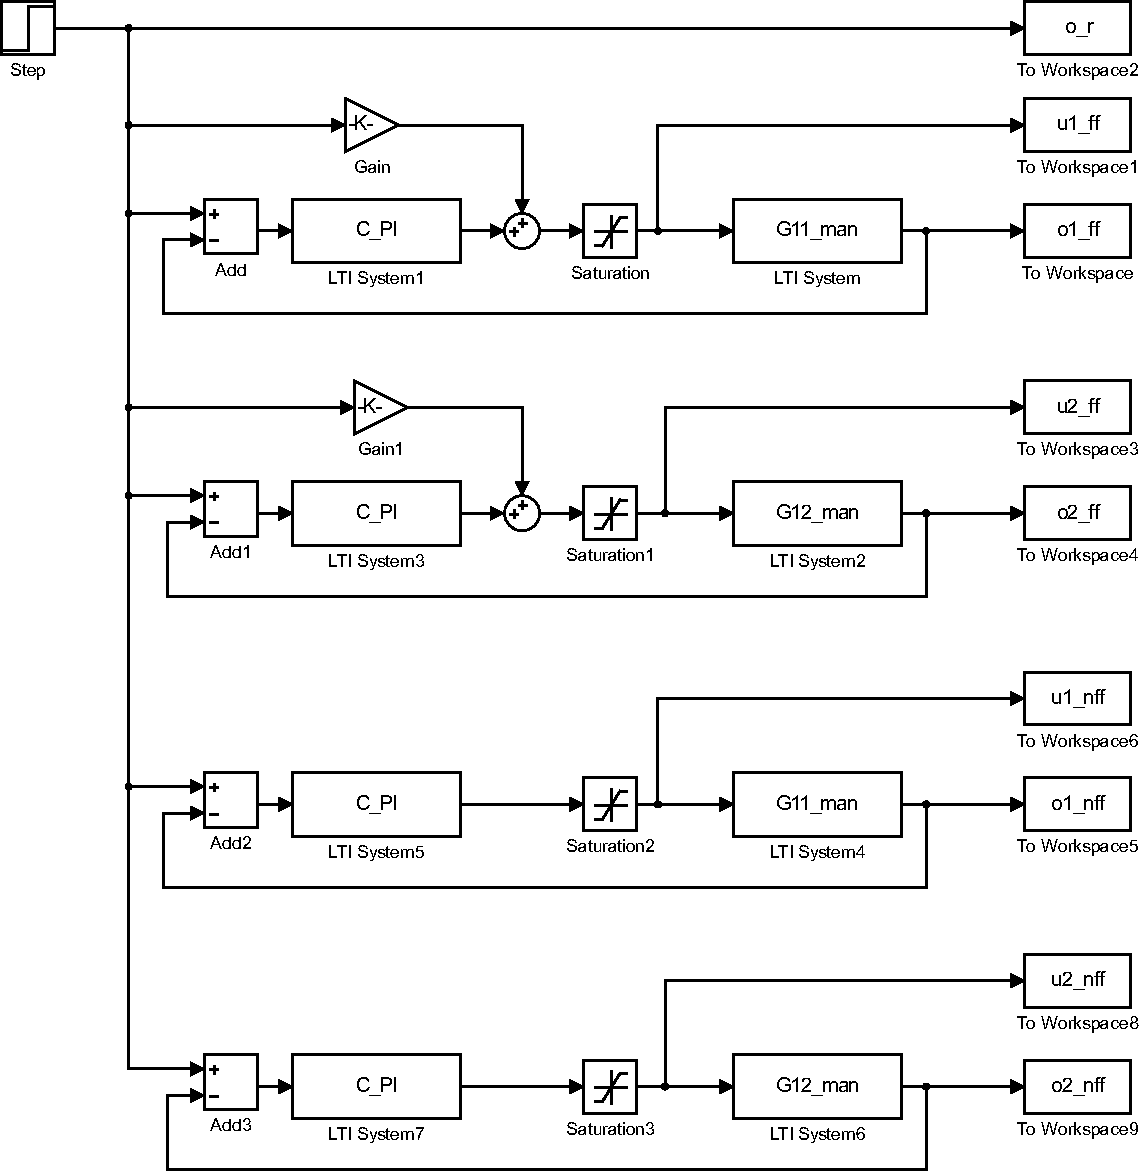
\includegraphics[width=0.8\textwidth]{13/model.pdf}
	\caption{Simulationsmodell des Regelkreises mit Vorsteuerung}
\end{figure}

\subsection{Simulation}

\lstinputlisting{13/simulation.m}

\begin{figure}[h!]
	\centering
	\begin{subfigure}{0.475\textwidth}
		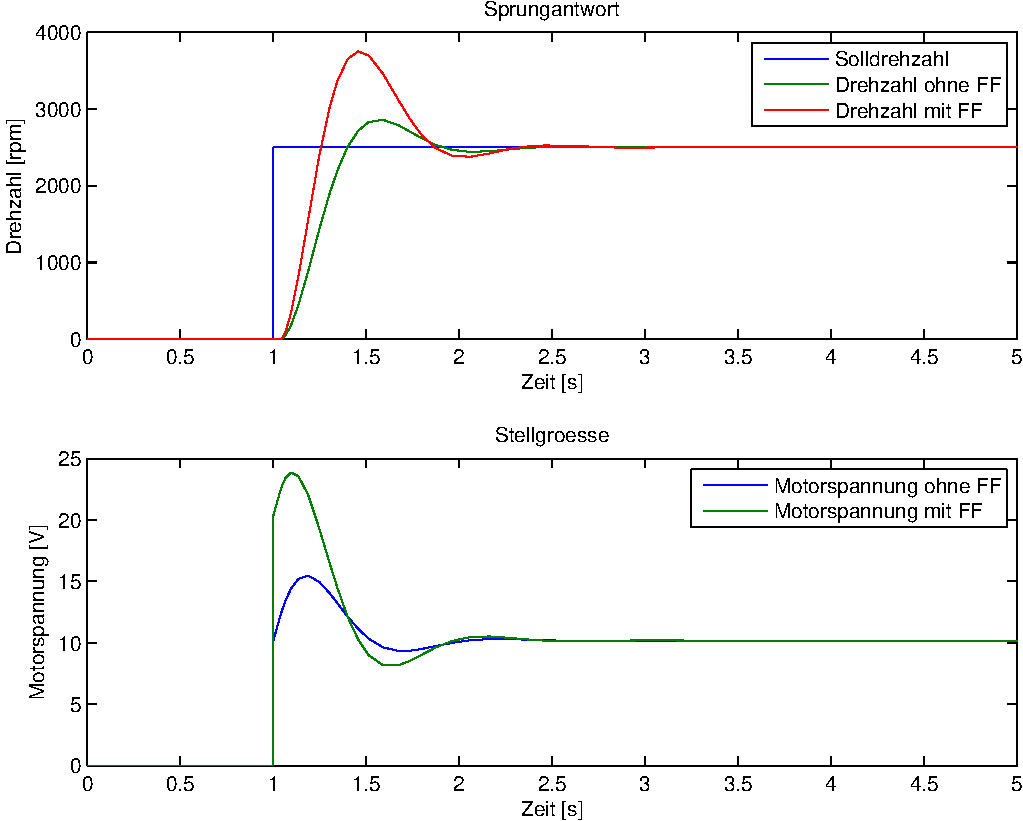
\includegraphics[width=1\textwidth]{13/step_noload.pdf}
		\caption{Sprungantwort ohne Bremse ($\alpha = 0$)}
	\end{subfigure}
	\hfill{}
	\begin{subfigure}{0.475\textwidth}
		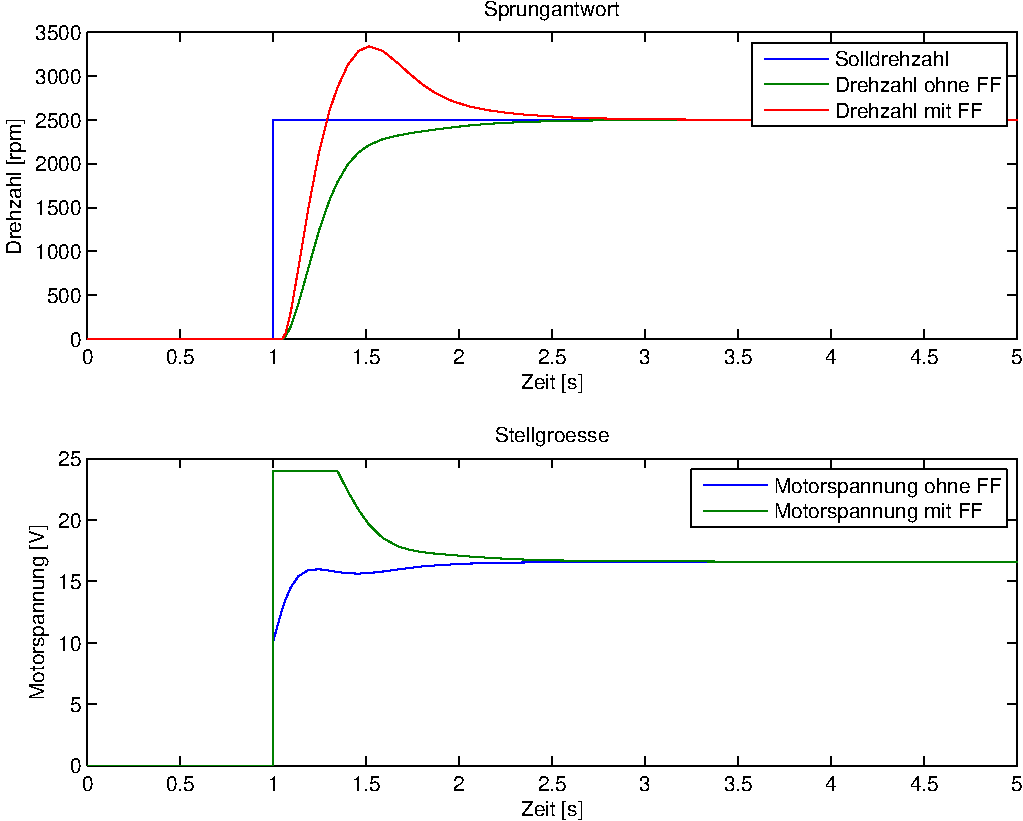
\includegraphics[width=1\textwidth]{13/step_load.pdf}
		\caption{Sprungantwort mit Bremse ($\alpha = 0.5$)}
	\end{subfigure}
	\caption{Vergleich der Sprungantworten mit und ohne Vorsteuerung}
\end{figure}
